% !TEX program = XeLaTeX
\documentclass[a4paper,conference]{IEEEtran}
\IEEEoverridecommandlockouts
% The preceding line is only needed to identify funding in the first footnote. If that is unneeded, please comment it out.
\usepackage{cite}
\usepackage[dvipdfmx]{graphicx}
\usepackage[dvipdfmx]{color}
\usepackage{float}
\usepackage{amsmath,amssymb,amsfonts}
%\usepackage{algorithmic}
\usepackage{textcomp}
\usepackage{lscape}
\usepackage{framed}
\usepackage{cleveref}
\usepackage{url}
%\usepackage{fontspec}
%\setmainfont{HaranoAjiMincho-Regular}

\usepackage{style/config}
\graphicspath{{./assets/}}
\begin{document}

\title{Intersection Crossing using Policy Optimization with Beta Distribution for Continuous Action}

\author{\IEEEauthorblockN{Kim Ang Kheang}
\IEEEauthorblockA{\textit{Graduate School of Science and Technology} \\
\textit{Niigata University}\\
Niigata, Japan \\
f21c501e@mail.cc.niigata-u.ac.jp}
\and
\IEEEauthorblockN{Tatsuya Yamazaki}
\IEEEauthorblockA{\textit{Faculty of Engineering} \\
\textit{Niigata University}\\
Niigata, Japan \\
yamazaki.tatsuya@ie.niigata-u.ac.jp}
}

\maketitle

%\begin{abstract}
%This document is a model and instructions for \LaTeX.
%This and the IEEEtran.cls file define the components of your paper [title, text, heads, etc.]. *CRITICAL: Do Not Use Symbols, Special Characters, Footnotes,
%or Math in Paper Title or Abstract.
%\end{abstract}

%\begin{IEEEkeywords}
%component, formatting, style, styling, insert
%\end{IEEEkeywords}

\section{Introduction}\label{sec:introduction}
Reinforcement Learning (RL) has emerged as a promising technique for autonomous driving applications, enabling agents to make decisions in dynamic environments. Efficiently navigating intersections is a critical challenge in this context, especially when dealing with continuous action spaces. Traditional RL methods often use Gaussian distributions~\cite{sutton2018reinforcement, capasso2021endtoend} for continuous actions, but they can have limitation.

To address this issue, we propose an innovative extension of the Proximal Policy Optimization (PPO) algorithm~\cite{schulman2017proximal} that leverages a Beta distribution. The Beta distribution offers more flexibility to model bounded action spaces~\cite{petrazzini2021proximal}, leading to better exploration and improved performance in intersection crossing tasks. Additionally, we introduce a duel channel neural architecture to accurately predict the $\alpha,\beta$ values of the Beta distribution, enhancing the agent's ability to sample actions effectively.

The choice of distribution in PPO can significantly impact the algorithm's performance. Utilizing the appropriate distribution, such as Beta for bounded action spaces, can lead to more efficient exploration, quicker convergence, and improved stability during training, whereas the wrong choice, like Gaussian for bounded actions, may result in suboptimal policies and hinder overall learning.

\section{Methodology}
We utilized the MetaDrive simulator~\cite{li2021metadrive}.
MetaDrive provides a realistic and dynamic environment for training and testing autonomous driving agent.

\subsection{Actor Network Architecture}
%\begin{figure}[H]
%    \centering
%    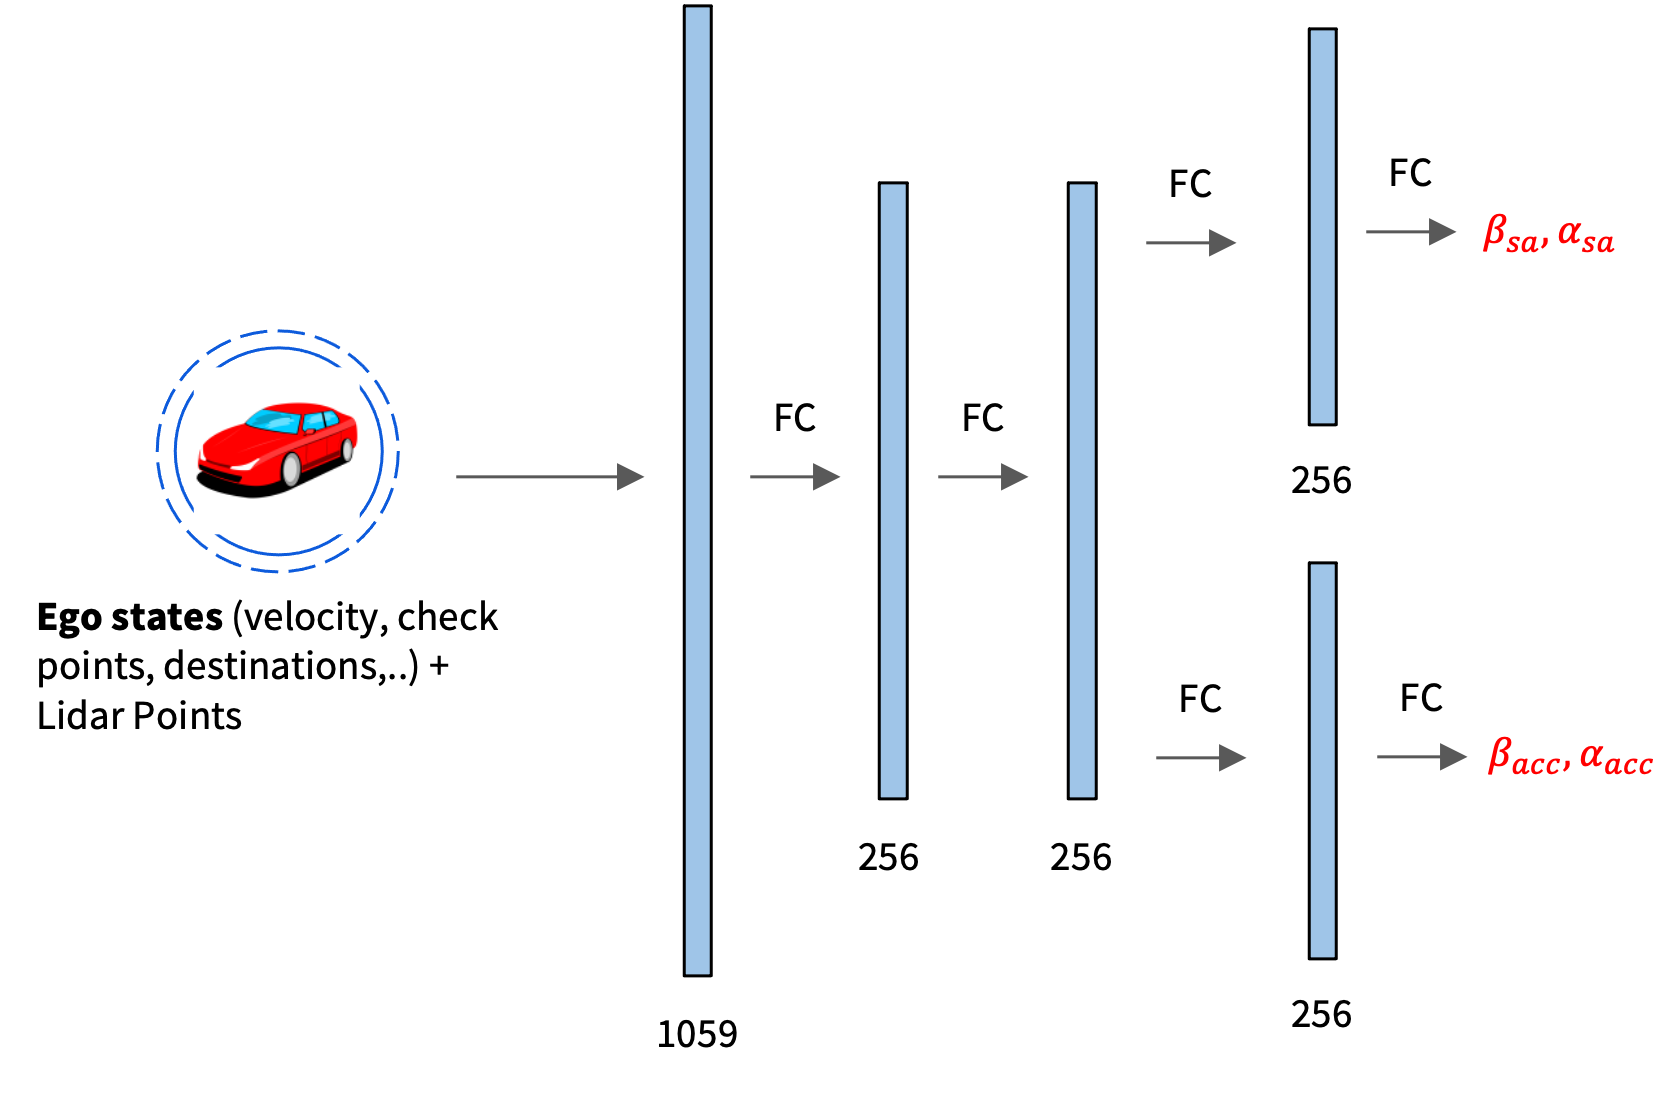
\includegraphics[width=6cm]{beta-policy.png}
%    \caption{Beta Policy Network Architecture}
%    \label{fig:beta-policy}
%\end{figure}
The actor network takes a sequential input of 1059 features, including ego state information, environment information, and Lidar cloud point data.
It consists of two hidden layers, each containing 256 neurons.
The output is then split into two fully connected layers to predict $\alpha,\beta$ values for acceleration and steering angle, respectively.

\subsection{Mapping to Action Space}
As the simulation environment accepts action with $a = [sa,acc]^T=[-1,1]^2$, the output from Beta's Probability Distribution Function is then mapped with the following equation:
\begin{equation}
    sa = 2h(\beta_{sa}, \alpha_{sa}) - 1\label{eq:equation5}
\end{equation}
\begin{equation}
    acc = 2h(\beta_{acc}, \alpha_{acc}) - 1\label{eq:equation6}
\end{equation}

\section{Result and Discussion}\label{sec:result-and-discussion}
\begin{figure}[H]
    \centering
    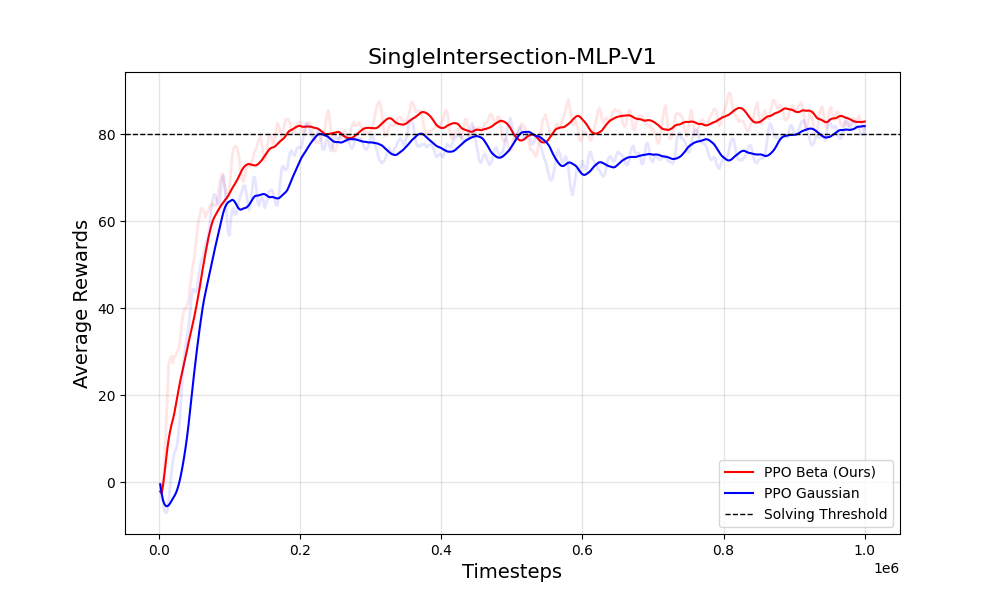
\includegraphics[width=9cm]{single-result.png}
    \caption{Beta Policy Network Architecture}\label{fig:figure}
\end{figure}
We implemented PPO with specific configurations: $\epsilon = 0.02$ (clipping parameter) and $\gamma = 0.99$ (discount factor). The environment solving threshold was set to 80 which means the agent can get through intersection successfully.

PPO Beta achieved the solving threshold faster and maintained higher average rewards throughout training compared to PPO Gaussian.
The utilization of the Beta distribution allowed PPO Beta to efficiently explore the continuous action space, leading to faster convergence and higher rewards.
\bibliographystyle{style/IEEEtran}
\bibliography{subdoc/reference}
\end{document}
